\chapter{Using the AWS Hadoop Streaming Interface}

\setcounter{problem}{1}

\section{Goal}

\begin{fullwidth}

Your goal in this lab is to learn how to launch a simple map-reduce job at Amazon using their elastic map reduce mechanism and the shell/commandline. Our application is the trite ``word counting,'' which we will use to find the most common words in a set of Google ads scarfed from the net in {\tt ads1000.txt} at github/parrt/msan501. You'll use Python as in the other labs.

\section{Discussion}

\subsection{Hadoop introduction}

{\em Hadoop} is a distributed computing framework that supports a \href{http://wiki.apache.org/hadoop/HadoopMapReduce}{\textcolor{blue}{map-reduce computing paradigm}}. The {\em map} operation executes on multiple machines and gets partial results, which are then combined with the {\em reduce} operation. 

Hadoop is written in Java and so, to use another language such as Python, we have to use the so-called {\em streaming interface}. That just means that we will write programs that read from standard input and write to standard output. 

The {\em Hadoop file system} (HDFS) is a distributed file system that can handle massive amounts of data by distributing it across multiple machines and hard drives. Hadoop tries to keep map operations on the machines that store the associated data the mappers should run on. That is what typically is done, but we will be using Amazons S3 storage instead since it is the easiest thing to do.

Hadoop splits the input into chunks and splits the chunks into lines before feeding the lines to standard input of the mappers. It gives each chunk of lines to a separate mapper task, which generates partial results. The mappers generate partial results as a set of key-value pairs of the form:

{\em key} \verb+\t+ {\em value} \verb+\n+

Because partial results are created on a variety of machines where the map tasks run, hadoop has to collect this data  from the machines of the cluster before giving it to the reducers. Hadoop sorts these partial results according to key (via merge sort) and distributes regions of the key space across one or more reducers. A specific key is only seen by a single reducer. A reducer reads these key-value pairs line by line from standard input and is responsible for generating a final result.  That output can be whatever we want, but in our case we will use the same key-value output format. 
We don't have to have any reducers at all, if we just want to run mappers across all the data.

We will be using Amazon Elastic MapReduce (EMR) that will take care of all the details of launching a cluster, running our job, and creating the output files.  A hadoop {\em job} is a chunk of work, which can have one or more tasks. If one of these tasks fails, hadoop tries to rerun them.  One of Hadoop's big benefits is that it is fault-tolerant. In a cluster of 1000 computers, it's very possible a machine will go down or the system operator will kick a power cord out by mistake. AWS introduces the notion of a {\em step}, which is one of more jobs.  We will not be using the step mechanism of the EMR GUI to launch jobs because, oddly enough, it's much easier and quicker to do it from the command line of the master node of the cluster.

Hadoop streaming generates an output file per reducer, which can be handy if we are interested in partitioning, say, sales results per country. In that case, we would have one reducer per country.  With three reducers, one per mapper, I got the following files in my S3 output folder:

\scalebox{.65}{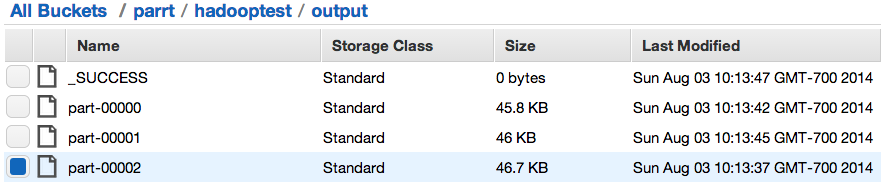
\includegraphics{figures/3reducers-output.png}}

To get a single output file, we need to specify a single reducer, which we will do below from the command line.

\subsection{Testing map-reduce on single machine}

Before spending money at Amazon to run your job, make sure that it works properly by simulating it from the command line on your laptop. To simulate hadoop collecting data and sending it as standard input to your mapper, we will use {\tt cat}:

\begin{lstlisting}[style=BashInputStyle]
$ cat /tmp/ads1000.txt
"title"	"blurb"	"url"	"target"	"retrievetime"
"Exclusive Music For DJs"	"DJ One Stop For Edits, Mash-Ups, Remixes. Browse, Listen, ...
...
\end{lstlisting}

 Then, pipe that input into the mapper (which will appear like standard input to the mapper: {\tt wcmap.py}):

\begin{lstlisting}[style=BashInputStyle]
$ cat /tmp/ads1000.txt | python wcmap.py
"title"	1
"blurb"	1
"url"	1
"target"	1
"retrievetime"	1
"Exclusive	1
Music	1
For	1
DJs"	1
"DJ	1
...
\end{lstlisting}

\noindent Hadoop always sorts the partial results coming out of each mapper before passing it to the reducer(s), which we can simulate bypassing the output of the mapper through {\tt sort}:

\begin{lstlisting}[style=BashInputStyle]
$ cat /tmp/ads1000.txt | python wcmap.py | sort
!	1
!	1
!	1
!	1
!	1
!"	1
!"	1
!"	1
!"	1
...
\end{lstlisting}

\noindent Obviously the data is not very interesting because we have not stripped out punctuation, which you can do as an exercise.  The point is that the data is sorted by key. Then, we can run the reduce job:

\begin{lstlisting}[style=BashInputStyle]
$ python wcmap.py < /tmp/ads1000.txt | sort | python wcreduce.py
...
\end{lstlisting}

\noindent The issue is that our Python program does not sort by keys when emitting key-value pairs, but we can use the command line to handle that. Here is our final command line that streams data using pipes between processes:

\begin{lstlisting}[style=BashInputStyle]
$ python wcmap.py < /tmp/ads1000.txt | sort | python wcreduce.py | sort
!       5
!"      6
"#3     3
"$189   3
"$200   1
...
\end{lstlisting}

\noindent We can also write that to file using:

\begin{lstlisting}[style=BashInputStyle]
$ python wcmap.py < /tmp/ads1000.txt | sort | python wcreduce.py | sort > output.txt
\end{lstlisting}

\noindent On a multicore machine, this process is virtually identical to what hadoop is doing for us, except of course on a smaller scale and without the network traffic.

\subsection{S3 storage}

AWS's elastic map reduce mechanism likes to process data out of its S3 storage. (It's tempting to try to process a local file with Hadoop from the cluster master, but that doesn't work as a local file is not available to slave nodes.) You will need to create a bucket in S3 that is unique across AWS so maybe use your user ID. My bucket is parrt. And I can access that with web address: \href{https://parrt.s3.amazonaws.com}{\textcolor{blue}{parrt.s3.amazonaws.com}}. As long as I've made the folders underneath public, then I can add elements to the URL to get access to those files. For example, here is the data that I have updated for our lab in the msan501 bucket:

\href{http://msan501.s3.amazonaws.com/data/ads1000.txt}{\textcolor{blue}{http://msan501.s3.amazonaws.com/data/ads1000.txt}}

You can load this data into your S3 bucket folder by downloading from msan501/data and uploading it into your own bucket.

In order to access S3 from the command line of the master server of your cluster, we first need to configure the {\tt aws} command with your \href{http://docs.aws.amazon.com/AWSSimpleQueueService/latest/SQSGettingStartedGuide/AWSCredentials.html}{\textcolor{blue}{access key and secret access key}}.

\begin{lstlisting}[style=BashInputStyle]
aws configure 
aws s3 ls s3://parrt/hadooptest/
aws s3 cp s3://parrt/hadooptest/output localdir --recursive
\end{lstlisting}

{\em Actually,  I can't get this to work yet as I can't figure out how to give it my .pem file, or whatever it means to resolve the following issue:} ``{\tt\small certificate routines:X509\_load\_cert\_crl\_file:system lib}''

\subsection{Launching a cluster}

From the EMR console at Amazon, click on the ``Create cluster'' button. Choose all the defaults on the resulting page, except:

\begin{itemize}
\item Turn OFF ``Termination protection'' near the top.
\item Set a log dir like {\tt s3://parrt/hadooptest/logs} or something appropriate.
\item You can delete Hive and Pig ``Applications to be installed'' as it slows down the launch and we aren't using  them for this lab.
\end{itemize}

\noindent The default is to use three machines, one master and two core. That's fine.

So, at the click of a button, we have a cluster up with everything installed properly to run Hadoop jobs!!!
 
\subsection{Running a Hadoop job}

On a cluster that has Hadoop installed, the easiest way to run a job is from the commandline shell. To demonstrate, we can use shell commands themselves as mappers and reducers:

\begin{lstlisting}[style=BashInputStyle]
$ hadoop jar /home/hadoop/contrib/streaming/hadoop-streaming.jar \
      -input s3://msan501/data/ads1000.txt \
      -output s3://parrt/hadooptest/output \
      -mapper /bin/cat \
      -reducer "/usr/bin/wc -l"	
\end{lstlisting}

\noindent Once the job finishes, you can go to the S3 console at AWS and look in your directory for the output. Your output files, part-0000*, will have one line with just a number like 330 in it. That is the result of running wc. After downloading from S3's web interface, I can look at the results with a simple command on my local machine:

\begin{lstlisting}[style=BashInputStyle]
$ cat ~/Downloads/part-0000[0-2]
330	
302	
368
\end{lstlisting}

\begin{center}
\fbox{\begin{minipage}{40em}
{\bf Warning!} If you launch a cluster and tell it to write output to an existing directory, it will fail with a permissions issue and the cluster will terminate.  Consequently, use output directories with different names for each run.
\end{minipage}}
\end{center}
~\\

Now let's run our Python code:

\begin{lstlisting}[style=BashInputStyle]
$ hadoop jar /home/hadoop/contrib/streaming/hadoop-streaming.jar \
    	-files s3://parrt/hadooptest/wcmap.py,s3://parrt/hadooptest/wcreduce.py \
    	-mapper wcmap.py \
    	-reducer wcreduce.py \
    	-input s3://msan501/data/ads1000.txt \
    	-output s3://parrt/hadooptest/output2
\end{lstlisting}

\noindent We can also run with the Python files locally if we copy them up. On your local machine, do this with the appropriate pem file:

\begin{lstlisting}[style=BashInputStyle]
$ scp -i ~/Dropbox/licenses/parrt.pem wc*.py \
    hadoop@ec2-54-87-142-212.compute-1.amazonaws.com:~hadoop
\end{lstlisting}

\noindent You will also need that certificate file to communicate with the slave machines so copy that pem file to the master as well:

\begin{lstlisting}[style=BashInputStyle]
$ scp -i ~/Dropbox/licenses/parrt.pem ~/Dropbox/licenses/parrt.pem \
    hadoop@ec2-54-87-142-212.compute-1.amazonaws.com:~hadoop/.ssh
\end{lstlisting}

\noindent On the master, set the permissions of that file as we did in a previous lab:

\begin{lstlisting}[style=BashInputStyle]
$ chmod 600 .ssh/parrt.pem
\end{lstlisting}

\noindent  Now that we have the Python code to the master, we need to copy the code to each of the slaves as the slaves will need to run the same code. To do that we need to know what the IP addresses of the slaves are:

\begin{lstlisting}[style=BashInputStyle]
$ hadoop dfsadmin -report | grep ^Name | cut -f2 -d:
DEPRECATED: Use of this script to execute hdfs command is deprecated.
Instead use the hdfs command for it.
10.110.197.20
10.206.58.80
$ scp -i .ssh/parrt.pem wc*.py hadoop@10.110.197.20:~hadoop
wcmap.py                                      100%  384     0.4KB/s   00:00    
wcreduce.py                                   100%  677     0.7KB/s   00:00    
$ scp -i .ssh/parrt.pem wc*.py hadoop@10.206.58.80:~hadoop
wcmap.py                                      100%  384     0.4KB/s   00:00    
wcreduce.py                                   100%  677     0.7KB/s   00:00    
\end{lstlisting}

\noindent Now, still on the master server, run the job without the {\tt -files} option:

\begin{lstlisting}[style=BashInputStyle]
$ hadoop jar /home/hadoop/contrib/streaming/hadoop-streaming.jar \
    	-mapper wcmap.py \
    	-reducer wcreduce.py \
    	-input s3://msan501/data/ads1000.txt \
    	-output s3://parrt/hadooptest/output2
\end{lstlisting}

\noindent To run with a single reducer instead of 3, use:

\begin{lstlisting}[style=BashInputStyle]
$ hadoop jar /home/hadoop/contrib/streaming/hadoop-streaming.jar \
    -D mapred.reduce.tasks=1 \
    -mapper wcmap.py \
    -reducer wcreduce.py \
    -input s3://msan501/data/ads1000.txt \
    -output s3://parrt/hadooptest/output3
\end{lstlisting}

 The output file will have a set of unsorted key-value pairs.

\subsection{Running a job via AWS web interface}

You can also run a job at Amazon without knowing the command line interface, but it's a lot of clicking. Here is the process:

\step Load your data into an S3 bucket folder by downloading from msan501/data and uploading it into your own bucket. Load your code into S3, presumably in a different folder.

\scalebox{.35}{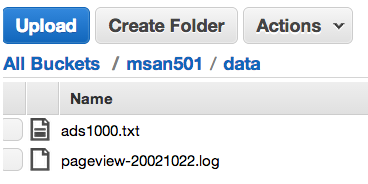
\includegraphics{figures/msan501-data.png}} \hspace{20pt}\scalebox{.30}{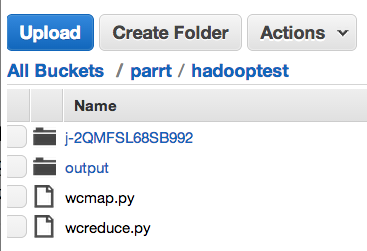
\includegraphics{figures/hadooptest.png}}

\step Create a cluster as shown previously and under ``Steps'' near the bottom, select ``Streaming program'' from the ``Add step'' drop-down. If you want to keep the cluster alive so that you can rerun jobs more quickly, set auto terminate to no. Otherwise set it to yes so that the cluster disappears after your job and you will not be charged further for it. 

\step Enter the fields of the step dialogue as shown, substituting your user ID or your bucket/folder names as appropriate:

\noindent\scalebox{0.85}{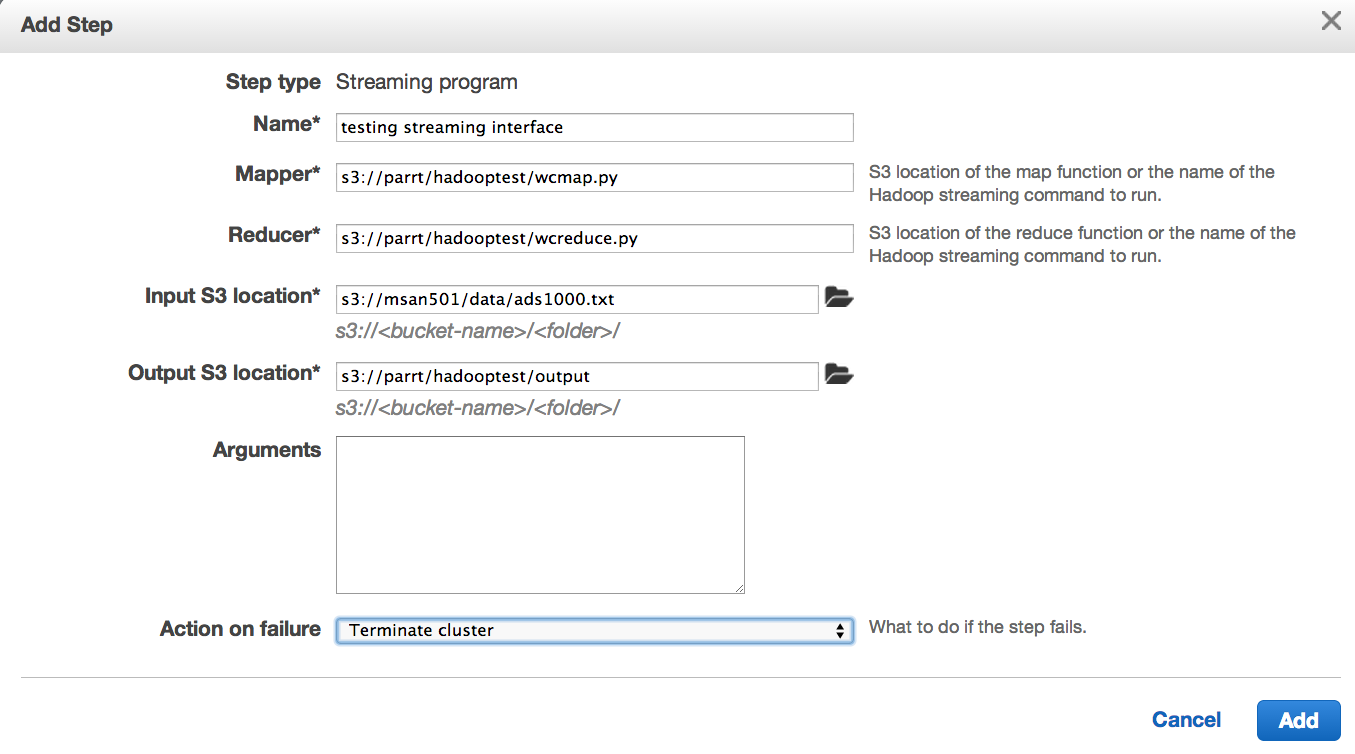
\includegraphics{figures/jobsetup.png}}

{\bf Warning!} If you launch a cluster and tell it to write output to an existing directory, it will fail with a permissions issue and the cluster will terminate.  Consequently, use output directories with different names for each run.

For convenience, here is the text so that you can cut-and-paste:

\begin{lstlisting}[style=BashInputStyle]
s3://parrt/hadooptest/wcmap.py
s3://parrt/hadooptest/wcreduce.py
s3://msan501/data/ads1000.txt
s3://parrt/hadooptest/output4
\end{lstlisting}

\step Wait about 15 minutes while Amazon creates the cluster and then wait a minute or so for your actual job to run.

\step Download or examine your data with the S3 interface.

Once our cluster is up, you can run another job ``quickly'' by adding another step. Go into EMR and select your cluster and then click "add step". That is a tiny link hidden down in the Steps area.  Or, run a command-line job.

\section{Extra credit}

Now that you know how to run a job, it's a good idea to spend the time improving the mapper so that it strips punctuation. That way we'll get a much better set of keys. You can also strip characters not in the printable ASCII code which will automatically strip non-English characters.

\section{Resources}

\begin{itemize}
\item You will find {\tt wcmap.py} and {\tt wcreduce.py} at msan501 github. There is also the necessary data file, {\tt ads1000.txt}.
\item \href{http://cs.smith.edu/dftwiki/index.php/Hadoop_Tutorial_3.2_--_Using_Your_Own_Streaming_WordCount_program}{\textcolor{blue}{A helpful tutorial}}, from which we get our sample programs.
\end{itemize}

\section{Deliverables}

None. Please follow along in class.

\end{fullwidth}
